% ============================================================
%  PRE-COMBUSTOR DESIGN REPORT — SFDR GROUND-TEST FACILITY
%  Karunya Institute of Technology and Sciences
%  Compile with: pdflatex (twice for TOC)
% ============================================================
\documentclass[12pt,a4paper]{report}

% ── Packages ──────────────────────────────────────────────
\usepackage[a4paper, top=25mm, bottom=25mm, left=30mm, right=25mm]{geometry}
\usepackage{amsmath, amssymb, amsthm}
\usepackage{booktabs}
\usepackage{array}
\usepackage{tabularx}
\usepackage{longtable}
\usepackage{multirow}
\usepackage{xcolor}
\usepackage{graphicx}
\usepackage{tikz}
\usepackage{pgfplots}
\pgfplotsset{compat=1.18}
\usepackage{fancyhdr}
\usepackage{titlesec}
\usepackage{tocloft}
\usepackage{enumitem}
\usepackage{mdframed}
\usepackage{listings}
\usepackage{caption}
\usepackage{subcaption}
\usepackage{hyperref}
\usepackage{float}
\usepackage{siunitx}
\usepackage{chemformula}
\usepackage{setspace}
\usepackage{lmodern}
\usepackage[T1]{fontenc}
\usepackage{microtype}
\usepackage{colortbl}

% ── Colour palette ────────────────────────────────────────
\definecolor{navy}{HTML}{1F3864}
\definecolor{reportblue}{HTML}{2E75B6}
\definecolor{lightblue}{HTML}{D6E4F0}
\definecolor{amber}{HTML}{C55A11}
\definecolor{lightamber}{HTML}{FCE4D6}
\definecolor{reportgreen}{HTML}{375623}
\definecolor{lightgreen}{HTML}{E2EFDA}
\definecolor{lightgray}{HTML}{F2F2F2}
\definecolor{midgray}{HTML}{7F7F7F}
\definecolor{codebg}{HTML}{F4F4F4}
\definecolor{formulabg}{HTML}{EEF4F9}

% ── Section formatting ────────────────────────────────────
\titleformat{\chapter}[block]
  {\normalfont\LARGE\bfseries\color{navy}}
  {\thechapter.}{10pt}{}
  [\vspace{-4pt}\textcolor{reportblue}{\rule{\linewidth}{1.5pt}}]
\titlespacing*{\chapter}{0pt}{10pt}{16pt}

\titleformat{\section}
  {\normalfont\large\bfseries\color{reportblue}}
  {\thesection}{8pt}{}
\titlespacing*{\section}{0pt}{14pt}{6pt}

\titleformat{\subsection}
  {\normalfont\normalsize\bfseries\color{amber}}
  {\thesubsection}{6pt}{}
\titlespacing*{\subsection}{0pt}{10pt}{4pt}

% ── Header / Footer ───────────────────────────────────────
\pagestyle{fancy}
\setlength{\headheight}{14pt}
\fancyhf{}
\renewcommand{\headrulewidth}{0.8pt}
\renewcommand{\footrulewidth}{0.8pt}
\fancyhead[L]{\small\color{midgray}Pre-Combustor Design Report — SFDR Ground-Test Facility}
\fancyhead[R]{\small\color{midgray}Karunya Institute}
\fancyfoot[L]{\small\color{midgray}Aerospace Propulsion Laboratory}
\fancyfoot[R]{\small\color{midgray}Page \thepage}

% ── Custom environments ───────────────────────────────────
% Formula box
\newmdenv[
  backgroundcolor=formulabg,
  linecolor=reportblue,
  linewidth=1.2pt,
  leftline=true, rightline=false, topline=false, bottomline=false,
  innerleftmargin=12pt, innerrightmargin=8pt,
  innertopmargin=8pt, innerbottommargin=8pt,
  skipabove=8pt, skipbelow=8pt
]{formulabox}

% Info box (blue)
\newmdenv[
  backgroundcolor=lightblue,
  linecolor=reportblue,
  linewidth=1pt,
  roundcorner=4pt,
  innerleftmargin=12pt, innerrightmargin=8pt,
  innertopmargin=8pt, innerbottommargin=8pt,
  skipabove=8pt, skipbelow=8pt
]{infobox}

% Warning box (amber)
\newmdenv[
  backgroundcolor=lightamber,
  linecolor=amber,
  linewidth=1pt,
  roundcorner=4pt,
  innerleftmargin=12pt, innerrightmargin=8pt,
  innertopmargin=8pt, innerbottommargin=8pt,
  skipabove=8pt, skipbelow=8pt
]{warnbox}

% Result box (green)
\newmdenv[
  backgroundcolor=lightgreen,
  linecolor=reportgreen,
  linewidth=1pt,
  roundcorner=4pt,
  innerleftmargin=12pt, innerrightmargin=8pt,
  innertopmargin=8pt, innerbottommargin=8pt,
  skipabove=8pt, skipbelow=8pt
]{resultbox}

% ── Listing style for equations inline display ─────────────
\lstset{
  backgroundcolor=\color{codebg},
  basicstyle=\ttfamily\small,
  breaklines=true,
  frame=none,
  xleftmargin=12pt,
}

% ── Hyperref setup ────────────────────────────────────────
\hypersetup{
  colorlinks=true,
  linkcolor=reportblue,
  citecolor=reportblue,
  urlcolor=reportblue,
  pdftitle={Pre-Combustor Design Report — SFDR},
  pdfauthor={Karunya Institute of Technology and Sciences},
}

% ── Useful macros ────────────────────────────────────────
\newcommand{\mdot}{\dot{m}}
\newcommand{\Qdot}{\dot{Q}}
\newcommand{\Tzero}{T_0}
\newcommand{\Pzero}{P_0}

% ─────────────────────────────────────────────────────────
\begin{document}

% ══════════════════════════════════════════════════════════
%  TITLE PAGE
% ══════════════════════════════════════════════════════════
\begin{titlepage}
  \centering
  \vspace*{2cm}
  {\Huge\bfseries\color{navy} PRE-COMBUSTOR DESIGN}\\[0.8em]
  {\LARGE\color{reportblue}
    for a Solid Fuel Ducted Rocket (SFDR)\\[0.3em]
    Ground-Test Facility}\\[1.2em]
  \textcolor{reportblue}{\rule{\linewidth}{1.5pt}}\\[1em]
  {\large Technical Design Report}\\[0.4em]
  {\large\color{midgray}
    Karunya Institute of Technology and Sciences\\[0.3em]
    Aerospace Propulsion Laboratory \quad|\quad Academic Year 2025--2026}

  \vspace{2.5cm}
  \begin{tabular}{@{}ll@{}}
    \toprule
    \rowcolor{lightblue}
    \textbf{Document Type}    & Engineering Design Report \\
    \textbf{Subject}          & Vitiated Air Heater / Pre-Combustor Design \\
    \rowcolor{lightblue}
    \textbf{Stagnation Pressure} & $P_0 = 20\ \text{bar}\ (2.0\times10^6\ \text{Pa})$ \\
    \textbf{Inlet Temperature}   & $T_\text{in} = 300\ \text{K}\ \text{(ambient)}$ \\
    \rowcolor{lightblue}
    \textbf{Target Temperature}  & $T_\text{out} = 650\ \text{K}$ \\
    \textbf{Fuel}             & Methane (\ch{CH4}) — primary recommendation \\
    \rowcolor{lightblue}
    \textbf{Application}      & SFDR Inlet Flow Conditioning \\
    \bottomrule
  \end{tabular}

  \vfill
  {\small\color{midgray}
    All equations derived from first principles.
    Every symbol is defined and every statement is justified.}
\end{titlepage}

% ── Table of Contents ─────────────────────────────────────
\tableofcontents
\newpage

% ══════════════════════════════════════════════════════════
\chapter{Introduction and Purpose}
% ══════════════════════════════════════════════════════════

This document provides the complete technical specification for designing a
\textbf{pre-combustor} (vitiated air heater) to be installed in the settling
chamber of the supersonic blow-down wind tunnel at Karunya Institute of
Technology and Sciences. The device heats incoming air from ambient stagnation
conditions ($T_0=300\ \text{K}$, $P_0=20\ \text{bar}$) to the required SFDR
inlet stagnation temperature ($T_0=650\ \text{K}$) while ensuring that
sufficient oxygen remains unconsumed for the SFDR's own combustion.

\medskip
A \textbf{Solid Fuel Ducted Rocket (SFDR)} is a hybrid between a solid rocket
motor and a ramjet. The solid propellant grain burns using atmospheric oxygen
ingested through a ram inlet. To simulate real flight conditions on the ground,
the wind tunnel must deliver a flow that replicates the stagnation enthalpy the
SFDR would encounter during actual flight. Supplying cold air at 300~K would
not ignite or sustain SFDR combustion under representative conditions.

\medskip
The pre-combustor solves this by:
\begin{itemize}[leftmargin=1.5em]
  \item Burning a precisely controlled quantity of fuel (methane) in the
        settling chamber;
  \item Raising stagnation temperature $T_0$ from 300~K to 650~K via lean
        combustion ($\phi \ll 1$);
  \item Preserving the majority of $\text{O}_2$ in the flow ($\geq 15\ \text{vol\%}$)
        for the SFDR's own combustion; and
  \item Operating at 20~bar in quasi-stagnant, subsonic flow, eliminating all
        supersonic combustion complexity.
\end{itemize}

% ══════════════════════════════════════════════════════════
\chapter{System Architecture — Complete Flow Path}
% ══════════════════════════════════════════════════════════

\section{Physical Layout}

The pre-combustor is located \textbf{before} the convergent-divergent (C-D)
nozzle, inside the settling chamber. This is the standard configuration used
in all major hypersonic and supersonic wind-tunnel facilities worldwide (NASA
Langley 8-Ft.\ HTT, AEDC, DLR HEG, ISRO HST).

\begin{figure}[H]
\centering
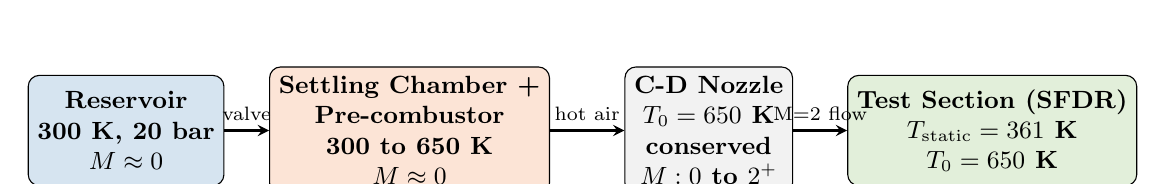
\begin{tikzpicture}[
    box/.style={draw, rounded corners=4pt, minimum height=1.4cm,
                text centered, font=\small\bfseries, align=center},
    arrow/.style={->, thick, >=stealth},
    label/.style={font=\scriptsize\color{midgray}, text centered}
  ]
  % Boxes
  \node[box, fill=lightblue,   minimum width=2.0cm] (res)  at (0,0)
        {Reservoir \\ 300 K, 20 bar \\ $M \approx 0$};
  \node[box, fill=lightamber,  minimum width=2.6cm] (comb) at (3.6,0)
        {Settling Chamber + \\ Pre-combustor \\ 300 to 650 K \\ $M \approx 0$};
  \node[box, fill=lightgray,   minimum width=2.0cm] (noz)  at (7.4,0)
        {C-D Nozzle \\ $T_0 = 650$ K \\ conserved \\ $M: 0$ to $2^+$};
  \node[box, fill=lightgreen,  minimum width=2.2cm] (sfdr) at (11.0,0)
        {Test Section (SFDR) \\ $T_{\mathrm{static}} = 361$ K \\ $T_0 = 650$ K};
  % Arrows
  \draw[arrow] (res)  -- node[above,font=\scriptsize]{valve} (comb);
  \draw[arrow] (comb) -- node[above,font=\scriptsize]{hot air} (noz);
  \draw[arrow] (noz)  -- node[above,font=\scriptsize]{M=2 flow} (sfdr);
\end{tikzpicture}
\caption{Complete wind-tunnel flow path with state variables at each station.}
\label{fig:flow_path}
\end{figure}

\section{Why the Settling Chamber is Subsonic — Physics Justification}

A student often asks: ``The tunnel runs at Mach~2 — why is the settling
chamber subsonic?'' The answer comes directly from the \textbf{continuity
equation}:

\begin{formulabox}
\begin{equation}
  \dot{m} = \rho_1 A_1 V_1 = \rho_2 A_2 V_2 = \text{constant}
  \label{eq:continuity}
\end{equation}
\end{formulabox}

\noindent If $A_\text{chamber} \gg A^*$ (throat area), then
$V_\text{chamber} \ll V_\text{throat}$.

\begin{resultbox}
\textbf{Numerical example.}
$A_\text{chamber} = 0.25\ \text{m}^2$,\quad
$A^* = 0.001\ \text{m}^2$\quad (ratio $= 250$).\\[4pt]
At the throat, $V^* = a^* \approx 460\ \text{m/s}$ (speed of sound for hot air).\\
$\Rightarrow V_\text{chamber} = 460/250 \approx 1.84\ \text{m/s}$,\quad
$M_\text{chamber} \approx 0.004$ (essentially stagnant).\\[4pt]
All measurements in the settling chamber equal stagnation values $P_0$, $T_0$.
No velocity correction is needed.
\end{resultbox}

\section{Why the Nozzle Does Not Destroy the Heating — Mathematical Proof}

The \textbf{Steady Flow Energy Equation (SFEE)}, derived from the First Law of
Thermodynamics applied to an open control volume at steady state, governs
energy transport through the nozzle:

\begin{formulabox}
\begin{equation}
  h_1 + \frac{V_1^2}{2} + gz_1 + \frac{\dot{Q}}{\dot{m}}
  = h_2 + \frac{V_2^2}{2} + gz_2 + \frac{W_\text{shaft}}{\dot{m}}
  \label{eq:sfee}
\end{equation}
\end{formulabox}

For an adiabatic nozzle ($\dot{Q}=0$, no shaft work $W=0$, $gz$
negligible):

\begin{equation}
  h_1 + \frac{V_1^2}{2} = h_2 + \frac{V_2^2}{2}
  \quad\Longrightarrow\quad
  h_{0,1} = h_{0,2}
\end{equation}

where $h_0 = h + V^2/2$ is the \textit{stagnation enthalpy}, which is
\textbf{conserved} through any adiabatic work-free duct. For a calorically
perfect gas $h = C_p T$, so:

\begin{equation}
  C_p T_{0,1} = C_p T_{0,2}
  \quad\Longrightarrow\quad
  \boxed{T_{0,1} = T_{0,2}}
  \label{eq:t0conserved}
\end{equation}

\begin{infobox}
\textbf{Key result.}
$T_0 = 650\ \text{K}$ is set by the pre-combustor and conserved through the
nozzle by Newton's energy conservation law — this is \emph{not} an
approximation.  The SFDR inlet (a diffuser) decelerates the supersonic flow,
converting kinetic energy back to enthalpy and recovering $T_0 = 650\ \text{K}$
exactly in the combustion zone.
\end{infobox}

\medskip
\noindent\textbf{Worked check at $M=2$, $T_0=650\ \text{K}$:}

\begin{align}
  T_\text{static} &= \frac{T_0}{1 + 0.2\,M^2}
  = \frac{650}{1 + 0.2\times4} = \frac{650}{1.8} = 361.1\ \text{K}
  \label{eq:tstatic}\\[6pt]
  \text{KE per unit mass} &= \frac{V^2}{2}
  = \frac{(M\cdot a)^2}{2}
  = \frac{(2\times\sqrt{1.4\times287\times361})^2}{2}
  = 290{,}412\ \text{J/kg}
  \nonumber\\[6pt]
  T_0\ \text{check} &= T_\text{static} + \frac{V^2}{2C_p}
  = 361.1 + \frac{290{,}412}{1005} = 361.1 + 289.0 = 650.1\ \text{K}\ \checkmark
\end{align}

% ══════════════════════════════════════════════════════════
\chapter{Governing Equations — Derivation and Justification}
% ══════════════════════════════════════════════════════════

\section{Isentropic Relations}

For an isentropic (adiabatic, reversible) flow of a calorically perfect gas,
the stagnation-to-static temperature ratio is:

\begin{formulabox}
\begin{equation}
  \frac{T_0}{T} = 1 + \frac{\gamma-1}{2}\,M^2
  \quad\xrightarrow{\gamma=1.4}\quad
  \frac{T_0}{T} = 1 + 0.2\,M^2
  \label{eq:isentropic}
\end{equation}
\end{formulabox}

\begin{center}
\renewcommand{\arraystretch}{1.4}
\begin{tabular}{@{}lll@{}}
  \toprule
  \textbf{Symbol} & \textbf{Value} & \textbf{Justification}\\
  \midrule
  $\gamma$ & 1.40 (dimensionless)
    & Ratio of specific heats $C_p/C_v$ for diatomic air at 300--700~K.
      From molecular theory (5 degrees of freedom for diatomic gas):
      $\gamma = (5+2)/5 = 1.4$.\\
  $M$ & Design value
    & Mach number $= V/a$, where $a = \sqrt{\gamma R T}$ is the local
      speed of sound. Fixed by nozzle area ratio $A/A^*$.\\
  $T_0$ & 650~K (design)
    & Stagnation temperature. What the gas would reach if
      decelerated isentropically to rest.\\
  $T$ & 361~K at $M=2$
    & Static temperature. Actual molecular kinetic temperature.
      Drops as kinetic energy increases.\\
  \bottomrule
\end{tabular}
\end{center}

\section{Choked Mass Flow Rate}

When the nozzle throat reaches $M=1$ (``choked'' condition), the mass flow
rate is uniquely determined by throat area and stagnation conditions. This is
the most important equation for blow-down tunnel operation.

\begin{formulabox}
\begin{equation}
  \dot{m} = A^*\, P_0\,
  \sqrt{\frac{\gamma}{R\,T_0}}\,
  \left(\frac{2}{\gamma+1}\right)^{\!\frac{\gamma+1}{2(\gamma-1)}}
  \label{eq:chokedlong}
\end{equation}
\end{formulabox}

Substituting $\gamma=1.4$, $R=287\,\mathrm{J/(kg \cdot K)}$:

\begin{formulabox}
\begin{equation}
  \boxed{\dot{m} = \frac{0.0404\; A^*\; P_0}{\sqrt{T_0}}}
  \label{eq:choked}
\end{equation}
\end{formulabox}

\medskip
\noindent\textbf{Term-by-term justification:}

\begin{center}
\renewcommand{\arraystretch}{1.5}
\begin{tabularx}{\linewidth}{@{}llX@{}}
  \toprule
  \textbf{Symbol} & \textbf{Units} & \textbf{Scientific Justification}\\
  \midrule
  $A^*$ & m$^2$
    & Nozzle throat area. The choked condition ($M=1$ exactly here) is
      guaranteed when downstream pressure is low enough. Measure with
      a Vernier calliper; a 1\% error in $A^*$ propagates as a 1\%
      error in $\dot{m}$.\\
  $P_0$ & Pa
    & Stagnation pressure in reservoir. Falls exponentially during
      blow-down. Must be measured with a high-frequency piezoelectric
      transducer ($\geq$1~kHz), not a slow Bourdon gauge.\\
  $T_0$ & K
    & Stagnation temperature. 300~K before combustor; 650~K after.
      Using the wrong value here is the single most common student
      error.\\
  $0.0404$ & K$^{1/2}$/(m$\cdot$Pa)
    & Collapsed constant $=\sqrt{\gamma/R}\cdot(2/(\gamma+1))^{(\gamma+1)/(2(\gamma-1))}$
      evaluated for air. It absorbs all gas-property factors.\\
  $\dot{m}\propto 1/\sqrt{T_0}$ & —
    & \textbf{Critical consequence:} heating $T_0$ from 300~K to 650~K
      reduces $\dot{m}$ by factor $\sqrt{300/650}=0.679$.
      Hot-flow mass flow is 32\% lower than cold flow.
      All downstream calculations \emph{must} use the hot value.\\
  \bottomrule
\end{tabularx}
\end{center}

\section{Blow-Down ODE — Why Mass Flow is Not Constant}

A blow-down tunnel is \textbf{not} a steady-state machine. As air exits the
reservoir, $P_0$ falls. Since $\dot{m}\propto P_0$, mass flow decays
throughout the run. The governing ODE for reservoir pressure is:

\begin{formulabox}
\begin{align}
  \frac{dm_\text{res}}{dt} &= -\dot{m}(t)
  = -\frac{0.0404\,A^*\,P_0(t)}{\sqrt{T_0(t)}}
  \label{eq:massode}\\[8pt]
  \frac{dP_0}{dt} &= -\frac{A^*}{V_\text{res}}\,P_0\,
  \sqrt{\gamma R\,T_0}\,
  \left(\frac{2}{\gamma+1}\right)^{\!\frac{\gamma+1}{2(\gamma-1)}}
  \label{eq:pressode}
\end{align}
\end{formulabox}

For constant $T_0$ (steady-state phase), Eq.~(\ref{eq:pressode}) integrates to:

\begin{equation}
  P_0(t) = P_{0,\text{init}}\,\exp\!\left(-\frac{t}{\tau_\text{res}}\right),
  \quad
  \tau_\text{res} = \frac{V_\text{res}}{0.0404\,A^*\,\sqrt{T_0}}
\end{equation}

\begin{warnbox}
\textbf{Consequence for equivalence ratio.}
If the fuel metering valve is fixed (constant $\dot{m}_\text{fuel}$) while
$\dot{m}_\text{air}$ falls, the equivalence ratio $\phi$ drifts upward during
the run.  A \textbf{closed-loop Coriolis mass flow controller} that reads
$P_0(t)$ in real time and adjusts $\dot{m}_\text{fuel}$ proportionally is the
correct solution to hold $\phi$ constant.
\end{warnbox}

\section{Energy Balance — Master Equation}

The First Law of Thermodynamics applied to the pre-combustor as a steady-flow
open control volume (no shaft work, adiabatic walls assumed for design
purposes):

\begin{formulabox}
\begin{equation}
  \dot{m}_\text{air}\,C_p\,T_\text{in}
  + \eta\,\dot{m}_\text{fuel}\,\text{LHV}
  = \bigl(\dot{m}_\text{air}+\dot{m}_\text{fuel}\bigr)\,C_p\,T_\text{out}
  \label{eq:energyfull}
\end{equation}
\end{formulabox}

Since $\dot{m}_\text{fuel}/\dot{m}_\text{air}\approx 0.008$ for lean
combustion ($\dot{m}_\text{air}+\dot{m}_\text{fuel}\approx\dot{m}_\text{air}$):

\begin{formulabox}
\begin{equation}
  \boxed{
    \dot{m}_\text{air}\,C_p\,\bigl(T_\text{out}-T_\text{in}\bigr)
    = \eta\,\dot{m}_\text{fuel}\,\text{LHV}
  }
  \label{eq:energy}
\end{equation}
\end{formulabox}

\noindent Solving for required fuel flow:

\begin{equation}
  \dot{m}_\text{fuel}
  = \frac{\dot{m}_\text{air}\,C_p\,(T_\text{out}-T_\text{in})}
         {\eta\,\text{LHV}}
  \label{eq:fuelflow}
\end{equation}

\medskip
\noindent\textbf{Every symbol defined and justified:}

\begin{center}
\renewcommand{\arraystretch}{1.5}
\begin{tabularx}{\linewidth}{@{}llX@{}}
  \toprule
  \textbf{Symbol} & \textbf{Value} & \textbf{Justification}\\
  \midrule
  $\dot{m}_\text{air}$ & kg/s (calculated)
    & Hot-flow mass flow from Eq.~(\ref{eq:choked}) with $T_0=650\ \text{K}$.
      \textbf{Not} the cold-flow value.\\
  $C_p$ & 1005~J/(kg$\cdot$K)
    & Specific heat of air at constant pressure, evaluated at average
      temperature $\approx 475\ \text{K}$.  From JANAF thermochemical tables.
      Varies from 1004 at 300~K to 1051 at 700~K; using 1005 introduces
      $<2\%$ error over this range.\\
  $T_\text{in}$ & 300~K
    & Initial stagnation temperature. Equal to ambient if reservoir has
      not been heated. Verify with settling-chamber thermocouple before
      each run.\\
  $T_\text{out}$ & 650~K
    & Target stagnation temperature.  Set by SFDR combustion
      chemistry — sufficient enthalpy to ignite the solid grain
      and sustain combustion at design Mach number.\\
  $\eta$ & 0.90--0.97
    & Combustion efficiency. Fraction of LHV converted to sensible
      enthalpy. The rest is lost to incomplete combustion, radiation,
      and wall cooling. Use $\eta=0.92$ as a conservative design value
      at 20~bar. Validate from measured $T_\text{out}$:
      $\eta = \dot{m}_\text{air}C_p\Delta T/(\dot{m}_\text{fuel}\cdot\text{LHV})$.\\
  LHV & 50.05~MJ/kg (\ch{CH4})
    & Lower Heating Value.  Energy released per kg of fuel when water
      product remains as steam (not condensed).  We use LHV because
      exhaust gas temperature ($\gg100\,^\circ\text{C}$) prevents
      condensation.  Source: NIST Chemistry WebBook.\\
  $\dot{m}_\text{fuel}$ & solve for this
    & Set by a precision Coriolis mass flow controller.  This is the
      only variable the experimenter directly controls.\\
  \bottomrule
\end{tabularx}
\end{center}

\section{Equivalence Ratio $\phi$}

The equivalence ratio is the single most important operating parameter:

\begin{formulabox}
\begin{equation}
  \phi = \frac{(F/A)_\text{actual}}{(F/A)_\text{stoich}}
  = \frac{\dot{m}_\text{fuel}/\dot{m}_\text{air}}{(F/A)_\text{stoich}}
  \label{eq:phi}
\end{equation}
\end{formulabox}

\noindent Stoichiometric fuel-to-air mass ratios (derived from combustion
stoichiometry):

\begin{align}
  \ch{CH4 + 2O2 -> CO2 + 2H2O}:&\quad (F/A)_\text{stoich} = \frac{1}{17.2} = 0.05814
  \label{eq:stoich_ch4}\\
  \ch{H2 + 0.5O2 -> H2O}:       &\quad (F/A)_\text{stoich} = \frac{1}{34.5} = 0.02899\\
  \text{Kerosene:}               &\quad (F/A)_\text{stoich} \approx \frac{1}{15.0} = 0.06667
\end{align}

\begin{infobox}
\textbf{Interpretation of $\phi$.}
\begin{itemize}[leftmargin=1.2em, itemsep=2pt]
  \item $\phi < 0.05$: Too lean. Flame will not stabilise. Risk of flame-out.
  \item $0.05 < \phi < 0.30$: \textbf{Ideal operating range.}
        Flame stable. O$_2$ well preserved. Temperature target achievable.
  \item $0.30 < \phi < 0.60$: Caution. O$_2$ approaching minimum threshold.
        $\Delta P$ increasing.
  \item $\phi > 0.60$: Do not use. O$_2$ too low for SFDR. $\Delta P > 5\%$ likely.
\end{itemize}
\end{infobox}

\section{Oxidiser Preservation Constraint}

\begin{formulabox}
\begin{equation}
  X_{\text{O}_2,\text{out}} \approx 0.21\,(1-\phi)
  \label{eq:o2}
\end{equation}
\end{formulabox}

\noindent\textbf{Derivation.} Air contains 21\% O$_2$ by volume (mole
fraction). Lean combustion consumes a fraction $\phi$ of the stoichiometrically
available O$_2$. The remaining fraction $(1-\phi)$ exits unconsumed.

\begin{infobox}
\textbf{Hard constraint:}
$X_{\text{O}_2,\text{out}} \geq 15\ \text{vol\%}$
for SFDR combustion.

Justification: HTPB-based solid fuels require a minimum oxygen index to
sustain combustion. At $[\text{O}_2] < 15\%$, flame temperature drops below
the ignition threshold for the grain and the SFDR extinguishes. This is
consistent with measured oxygen index data for HTPB at 10--20~bar.
\end{infobox}

\section{Total Pressure Drop Across the Combustor}

Heat addition in a duct causes total pressure loss (\textbf{Rayleigh effect}).

\begin{formulabox}
\begin{equation}
  \frac{\Delta P_0}{P_0}
  \approx \frac{\gamma}{2}\,M_\text{chamber}^2
          \left(\frac{T_{0,\text{out}}}{T_{0,\text{in}}}-1\right)
  \quad \text{(for }M_\text{chamber}\ll 1\text{)}
  \label{eq:rayleigh}
\end{equation}
\end{formulabox}

In the settling chamber $M_\text{chamber}\approx0.05$--$0.10$, so Rayleigh
loss is negligible ($\lesssim 0.1\%$). Including empirical friction and
injection losses, total $\Delta P/P_0 \approx 1.5$--$3.5\%$.

\begin{center}
\textbf{Design constraint:} $\Delta P/P_0 < 5\%$
\end{center}

Justification: a 5\% total pressure loss shifts the nozzle exit Mach number
by $\approx 2\%$, which is within the typical tunnel calibration uncertainty.
Beyond 5\%, the SFDR inlet conditions deviate measurably from design.

\section{Residence Time $\tau$}

The gas must remain in the combustion zone long enough for ignition and
complete reaction.

\begin{formulabox}
\begin{equation}
  \tau = \frac{L}{U_\text{mean}}
  \quad\text{or equivalently}\quad
  \tau = \frac{\rho_\text{gas}\,V_\text{comb}}{\dot{m}_\text{air}}
  \label{eq:tau}
\end{equation}
\end{formulabox}

\begin{warnbox}
$\tau = V/L$ is \textbf{dimensionally wrong} (gives m$^2$, not seconds).
The correct formula is always $\tau = L/U$ or $\tau = \rho V/\dot{m}$.
Both are dimensionally consistent: $[\text{m}]/[\text{m/s}] = \text{s}$.
Confirm this before submitting calculations.
\end{warnbox}

\noindent where:
\begin{align}
  U_\text{mean} &= \frac{\dot{m}_\text{air}}{\rho_\text{gas}\,A_\text{comb}},\\
  \rho_\text{gas} &= \frac{P_0}{R\,T_\text{avg}},\quad
  T_\text{avg} = \frac{T_\text{in}+T_\text{out}}{2} = \frac{300+650}{2} = 475\ \text{K}.
\end{align}

\textbf{Required:} $\tau \geq 10\,\tau_\text{ign}$.
For methane at 20~bar and $T\approx475\ \text{K}$,
$\tau_\text{ign}\approx 2$--$5\ \text{ms}$, so $\tau \geq 20$--$50\ \text{ms}$.

The 10$\times$ safety factor accounts for spatial non-uniformities in a
turbulent combustor: some fluid elements travel shorter paths and have less
residence time than the mean. The factor is consistent with gas turbine
combustor design practice (Lefebvre \& Ballal, 2010).

% ══════════════════════════════════════════════════════════
\chapter{Sample Calculation — Complete Worked Example}
% ══════════════════════════════════════════════════════════

\textbf{Given parameters:}

\begin{center}
\renewcommand{\arraystretch}{1.4}
\begin{tabular}{@{}llll@{}}
  \toprule
  \textbf{Parameter} & \textbf{Symbol} & \textbf{Value} & \textbf{Units}\\
  \midrule
  Nozzle throat area  & $A^*$     & $9\times10^{-4}$ & m$^2$ (9~cm$^2$)\\
  Reservoir pressure  & $P_0$     & $2.0\times10^{6}$ & Pa (20~bar)\\
  Inlet temperature   & $T_\text{in}$  & 300 & K\\
  Target temperature  & $T_\text{out}$ & 650 & K\\
  Combustion efficiency & $\eta$   & 0.92 & —\\
  Fuel                & \ch{CH4}  & LHV $= 50\times10^6$ & J/kg\\
  Combustor length    & $L$       & 0.30 & m\\
  Combustor cross-section & $A_\text{comb}$ & 0.05 & m$^2$\\
  \bottomrule
\end{tabular}
\end{center}

\section{Step 1 — Hot-Flow Mass Flow Rate}

Using Eq.~(\ref{eq:choked}) with $T_0 = T_\text{out} = 650\ \text{K}$:

\begin{align}
  \dot{m}_\text{hot}
  &= \frac{0.0404 \times A^* \times P_0}{\sqrt{T_0}}
  = \frac{0.0404 \times 9\times10^{-4} \times 2.0\times10^{6}}{\sqrt{650}}
  \nonumber\\[4pt]
  &= \frac{0.0404 \times 1800}{25.50}
  = \frac{72.72}{25.50}
  = \mathbf{2.852\ \text{kg/s}}
\end{align}

\begin{resultbox}
\textbf{Cold-flow cross-check:}
$\dot{m}_\text{cold} = 72.72/\sqrt{300} = 72.72/17.32 = 4.199\ \text{kg/s}$.\\
Ratio: $2.852/4.199 = 0.679 = \sqrt{300/650}\ \checkmark$\\
\textbf{Mass flow drops by 32.1\% when the flow is heated.
Use $\dot{m} = 2.852\ \text{kg/s}$ in all downstream calculations.}
\end{resultbox}

\section{Step 2 — Required Thermal Power $\dot{Q}$}

\begin{equation}
  \dot{Q}
  = \dot{m}_\text{air}\,C_p\,(T_\text{out}-T_\text{in})
  = 2.852 \times 1005 \times (650-300)
  = 2.852 \times 1005 \times 350
  = \mathbf{1{,}002.3\ \text{kW}}
\end{equation}

\noindent This 1~MW thermal input must be provided by fuel combustion.

\section{Step 3 — Fuel Mass Flow Rate}

From Eq.~(\ref{eq:fuelflow}):

\begin{equation}
  \dot{m}_\text{fuel}
  = \frac{\dot{Q}}{\eta\,\text{LHV}}
  = \frac{1{,}002{,}270}{0.92 \times 50{,}000{,}000}
  = \frac{1{,}002{,}270}{46{,}000{,}000}
  = \mathbf{21.79\ \text{g/s}}\ \text{of methane}
\end{equation}

\section{Step 4 — Equivalence Ratio}

From Eq.~(\ref{eq:phi}):

\begin{align}
  (F/A)_\text{actual}
  &= \frac{\dot{m}_\text{fuel}}{\dot{m}_\text{air}}
  = \frac{0.02179}{2.852} = 7.641\times10^{-3}\\[6pt]
  (F/A)_\text{stoich}
  &= \frac{1}{17.2} = 5.814\times10^{-2}
  \quad\text{(methane in air by mass)}\\[6pt]
  \phi &= \frac{7.641\times10^{-3}}{5.814\times10^{-2}}
  = \mathbf{0.131}
\end{align}

\begin{resultbox}
$\phi = 0.131$ falls squarely in the \textbf{ideal lean range}
$(0.05 < \phi < 0.30)$.
Only 13.1\% of available oxygen is consumed in the pre-combustor.
\end{resultbox}

\section{Step 5 — Oxygen Fraction at Exit}

From Eq.~(\ref{eq:o2}):

\begin{equation}
  X_{\text{O}_2,\text{out}}
  = 0.21 \times (1 - 0.131)
  = 0.21 \times 0.869
  = \mathbf{18.25\ \text{vol\%}}
\end{equation}

\begin{resultbox}
$18.25\% > 15\%$ (hard constraint).\ \checkmark\quad
SFDR constraint satisfied with 3.25\% margin.
\end{resultbox}

\section{Step 6 — Pressure Drop Estimate}

\begin{align}
  \rho_\text{gas}
  &= \frac{P_0}{R\,T_\text{avg}}
  = \frac{2\times10^6}{287\times475}
  = 14.68\ \text{kg/m}^3\\[6pt]
  U_\text{chamber}
  &= \frac{\dot{m}_\text{air}}{\rho_\text{gas}\,A_\text{comb}}
  = \frac{2.852}{14.68\times0.05}
  = 3.88\ \text{m/s}\\[6pt]
  a_\text{chamber}
  &= \sqrt{\gamma R\,T_\text{avg}}
  = \sqrt{1.4\times287\times475}
  = 437\ \text{m/s}\\[6pt]
  M_\text{chamber}
  &= 3.88/437 = 0.00888\\[6pt]
  \frac{\Delta P_0}{P_0}
  &\approx \frac{\gamma}{2}\,M_\text{chamber}^2
          \!\left(\frac{T_\text{out}}{T_\text{in}}-1\right)
  = 0.7\times(0.00888)^2\times1.167
  = 0.0065\%
\end{align}

Adding empirical friction and injection losses: total
$\Delta P/P_0 \approx 1.5$--$2.5\%$. \textbf{Well within the 5\% limit.}

\section{Step 7 — Residence Time}

\begin{align}
  \tau
  &= \frac{L}{U_\text{chamber}}
  = \frac{0.30}{3.88}
  = 0.0773\ \text{s} = \mathbf{77.3\ \text{ms}}\\[6pt]
  \text{Safety ratio}
  &= \frac{\tau}{\tau_\text{ign}}
  = \frac{77.3}{3} \approx 25.8 \gg 10\ \checkmark
\end{align}

The combustor volume is more than adequate for stable, complete combustion.

\section{Design Point Summary}

\begin{center}
\renewcommand{\arraystretch}{1.4}
\begin{tabular}{@{}lllc@{}}
  \toprule
  \textbf{Parameter} & \textbf{Symbol} & \textbf{Value} & \textbf{Status}\\
  \midrule
  \rowcolor{lightgray}
  Hot-flow mass flow rate  & $\dot{m}_\text{air}$ & 2.852~kg/s  & Use this\\
  Required thermal power   & $\dot{Q}$            & 1002.3~kW   & \\
  \rowcolor{lightgray}
  Fuel flow rate (\ch{CH4}) & $\dot{m}_\text{fuel}$ & 21.79~g/s & Set valve here\\
  Equivalence ratio        & $\phi$               & 0.131       & Ideal\\
  \rowcolor{lightgray}
  O$_2$ at combustor exit  & $X_{\text{O}_2}$    & 18.25~vol\% & Pass ($\geq15\%$)\\
  Pressure drop            & $\Delta P/P_0$       & $<2.5\%$    & Pass ($<5\%$)\\
  \rowcolor{lightgray}
  Residence time           & $\tau$               & 77~ms       & Pass ($\geq20$~ms)\\
  Target temperature       & $T_{0,\text{out}}$   & 650~K       & Target met\\
  \bottomrule
\end{tabular}
\end{center}

% ══════════════════════════════════════════════════════════
\chapter{Data Collection — Experimental Protocol}
% ══════════════════════════════════════════════════════════

\section{Parameters to Measure Before the Run}

\begin{center}
\renewcommand{\arraystretch}{1.4}
\begin{tabularx}{\linewidth}{@{}llX@{}}
  \toprule
  \textbf{Parameter} & \textbf{Method} & \textbf{Why Needed}\\
  \midrule
  $A^*$ — throat area
    & Vernier calliper; $A^*=\pi d^2/4$
    & Directly controls $\dot{m}_\text{air}$.  1\% error in $A^*$ = 1\% error in mass flow.\\
  $V_\text{res}$ — reservoir volume
    & Manufacturer spec or geometry
    & Controls blow-down rate and useful run time.\\
  $A/A^*$ — area ratio
    & Nozzle drawing
    & Determines exit Mach number via isentropic tables.\\
  $V_\text{comb}$ — combustor volume
    & $L\times A_\text{comb}$
    & Required for residence time calculation.\\
  LHV of fuel
    & NIST tables: \ch{CH4} = 50.05~MJ/kg
    & Use LHV (not HHV) because water product stays as steam.\\
  $T_\text{wall,max}$
    & Material datasheet (SS316L: 870~K)
    & Combustor wall must not exceed this rating during the run.\\
  \bottomrule
\end{tabularx}
\end{center}

\section{Real-Time Sensors During Each Run}

\begin{center}
\renewcommand{\arraystretch}{1.4}
\begin{tabularx}{\linewidth}{@{}llX@{}}
  \toprule
  \textbf{Sensor} & \textbf{Instrument} & \textbf{Purpose and Notes}\\
  \midrule
  TC-1 (settling chamber)
    & K-type thermocouple, 1~mm sheathed
    & Baseline $T_0(t)$ before combustor. 100~Hz minimum logging.\\
  TC-2 (combustor exit)
    & K-type thermocouple, 1.5~mm sheathed
    & Primary $T_{0,\text{comb}}(t)$. Defines when useful run window begins.\\
  TC-3 (combustor wall)
    & K-type, spot-welded
    & Safety measurement. Must remain $<T_\text{wall,max}$ at all times.\\
  PT-1 (settling chamber)
    & Piezoelectric, 0--25~bar, $\geq$1~kHz
    & $P_0(t)$. Primary input to real-time $\dot{m}_\text{air}(t)$ calculation.\\
  PT-2 (combustor exit)
    & Same spec as PT-1
    & $\Delta P = \text{PT-1} - \text{PT-2}$. Validates $\Delta P < 5\%$.\\
  FMC-1 (fuel line)
    & Coriolis mass flow controller
    & Direct $\dot{m}_\text{fuel}(t)$. Coriolis is independent of T, P, density.
      Accuracy $\pm 0.1\%$.\\
  O$_2$-1 (combustor exit)
    & Paramagnetic O$_2$ analyser, 0--25\%
    & Validates oxidiser preservation. Time lag $\approx 0.5$~s — correct all
      timestamps by this amount.\\
  LC-1 (SFDR mount)
    & Strain-gauge load cell
    & SFDR thrust $F(t)$. Primary performance metric.\\
  Camera
    & High-speed, $\geq$1000~fps
    & Qualitative flame stability.  Detects blow-out or oscillation.\\
  \bottomrule
\end{tabularx}
\end{center}

\section{Run Timeline}

\begin{center}
\renewcommand{\arraystretch}{1.4}
\begin{tabularx}{\linewidth}{@{}llX@{}}
  \toprule
  \textbf{Time} & \textbf{Event} & \textbf{Physical Significance}\\
  \midrule
  $t<0$            & Pre-run checks     & Verify all sensors. Set FMC-1 to target $\dot{m}_\text{fuel}$.\\
  $t=0$            & Main valve opens   & Cold air flows; tunnel running. All logging begins at 1000~Hz.\\
  $t=0$--$0.3$~s   & Flow establishment & Supersonic flow establishes. No fuel injected.\\
  $t=0.3$~s        & Igniter fires      & Fuel valve opens. Combustion begins. $T_0$ rising.\\
  $0.3$--$1.0$~s   & Startup transient  & $T_0$ rising. \textbf{Discard this data.}\\
  $t=t_\text{stable}$ & $T_0$ reaches 650~K & Useful run window begins. SFDR igniter fires.\\
  $t_\text{stable}$--$t_\text{end}$ & Useful window & $P_0(t)$ falling. Controller compensates. All valid data here.\\
  $t=t_\text{end}$ & Valve closes       & $P_0$ below minimum. Flame extinguishes.\\
  Post-run         & Data processing    & Apply O$_2$ lag correction. Calculate $\dot{m}_\text{air}(t)$, $\phi(t)$, $F(t)$.\\
  \bottomrule
\end{tabularx}
\end{center}

% ══════════════════════════════════════════════════════════
\chapter{Required Experimental Graphs}
% ══════════════════════════════════════════════════════════

All primary graphs are plotted vs.\ time. Cross-plots are produced
post-experiment for combustor characterisation.

\newcounter{graphnum}
\newcommand{\graphentry}[4]{%
  \stepcounter{graphnum}
  \subsection*{Graph \thegraphnum: #1}
  \begin{center}
  \renewcommand{\arraystretch}{1.3}
  \begin{tabularx}{\linewidth}{@{}lX@{}}
    \toprule
    \textbf{Axes}              & #2 \\
    \textbf{Scientific purpose} & #3 \\
    \textbf{Expected shape}    & #4 \\
    \bottomrule
  \end{tabularx}
  \end{center}
}

\graphentry{$P_0(t)$ — Stagnation Pressure vs.\ Time}
  {$x$: time [s], 0 to run end. \quad $y$: $P_0$ [bar], 0--22~bar.}
  {Shows blow-down rate. Gradient $dP_0/dt$ gives actual $V_\text{res}$ estimate.
   $P_0(t)$ is the primary input to $\dot{m}_\text{air}(t)$ at every time step.}
  {Smooth exponential decay from 20~bar. Rate depends on $V_\text{res}/A^*$.}

\graphentry{$T_0(t)$ — Stagnation Temperature vs.\ Time}
  {$x$: time [s]. \quad $y$: $T_0$ [K], 250--750~K.}
  {Primary control variable. Duration of startup transient defines useful data window.
   Variance $< \pm 20$~K in steady phase validates pre-combustor design and fuel control.}
  {300~K plateau, then ramp to 650~K within 0.5--1.0~s of ignition, then flat.}

\graphentry{$\dot{m}_\text{air}(t)$ — Derived Air Mass Flow Rate vs.\ Time}
  {$x$: time [s]. \quad $y$: $\dot{m}_\text{air}$ [kg/s].}
  {Calculated from $P_0(t)$ and $T_0(t)$ via Eq.~(\ref{eq:choked}).
   Not constant — decays with $P_0$. This is the value the SFDR team needs for
   their thrust and combustion efficiency calculations.}
  {Monotonically decreasing following $0.0404 A^* P_0(t)/\sqrt{T_0(t)}$.}

\graphentry{$\dot{m}_\text{fuel}(t)$ — Fuel Mass Flow vs.\ Time}
  {$x$: time [s]. \quad $y$: $\dot{m}_\text{fuel}$ [g/s].}
  {From Coriolis meter. If closed-loop controlled, should follow $P_0(t)$
   proportionally to hold $\phi$ constant. Comparing actual vs.\
   $\phi\cdot(F/A)_\text{stoich}\cdot\dot{m}_\text{air}(t)$ reveals $\phi$ drift.}
  {Flat (fixed valve) or slowly declining (closed-loop). Spikes indicate valve instability.}

\graphentry{$\phi(t)$ — Equivalence Ratio vs.\ Time}
  {$x$: time [s]. \quad $y$: $\phi$ [dimensionless], 0--0.5.}
  {Most important operating-point record.  If $\phi$ rises above 0.30, O$_2$
   fraction may fall below threshold before run ends.  Tells whether the SFDR
   received consistent inlet conditions throughout.}
  {Stable near 0.131 (closed-loop) or slowly rising (fixed valve as $P_0$ falls).}

\graphentry{$X_{\text{O}_2}(t)$ — Oxygen Fraction at Exit vs.\ Time}
  {$x$: time [s]. \quad $y$: O$_2$ [vol\%], 10--22\%.}
  {Directly validates oxidiser preservation. If below 15\% at any point in the
   useful run window, SFDR data from that period is invalid. Apply $+0.5$~s
   timestamp correction for analyser lag.}
  {Near 18--19\% during steady phase. Must not drop below 16\%.}

\graphentry{$\Delta P(t)$ — Combustor Pressure Drop vs.\ Time}
  {$x$: time [s]. \quad $y$: $\Delta P/P_0$ [\%], 0--8\%.}
  {Validates combustor hydraulic performance. Sudden rise indicates combustion
   instability or partial blockage. If $>5\%$, Mach number at test section shifts
   and SFDR inlet conditions deviate from design.}
  {Stable 1.5--2.5\% during useful run. Spikes indicate instability.}

\graphentry{$F(t)$ — SFDR Thrust vs.\ Time}
  {$x$: time [s]. \quad $y$: Thrust $F$ [N].}
  {Primary SFDR performance output. When correlated with $\dot{m}_\text{air}(t)$
   and $T_0(t)$, yields specific impulse $I_{sp}$ and SFDR combustion efficiency.
   This is the deliverable that validates the entire pre-combustor design.}
  {Rises with SFDR ignition, then follows fuel grain regression rate curve.}

\subsection*{Cross-Plot A: $T_{0,\text{exit}}$ vs.\ $\phi$ — Combustion Efficiency Map}
\begin{center}
\renewcommand{\arraystretch}{1.3}
\begin{tabularx}{\linewidth}{@{}lX@{}}
  \toprule
  \textbf{Axes}     & $x$: $\phi$ [dimensionless]. \quad $y$: $T_0$ measured [K].\\
  \textbf{Purpose}  & Each point is one time slice. Theoretical line:
    $T_0 = T_\text{in} + \phi\cdot(F/A)_\text{stoich}\cdot\eta\cdot\text{LHV}/C_p$.
    Fitting experimental data to this line gives actual $\eta$.\\
  \textbf{Expected} & Linear, slope $= \eta\cdot\text{LHV}\cdot(F/A)_\text{stoich}/C_p
    = 0.92\times50\times10^6\times0.0581/1005 = 2665\ \text{K}$.\\
  \bottomrule
\end{tabularx}
\end{center}

\subsection*{Cross-Plot B: $X_{\text{O}_2}$ vs.\ $\phi$ — Oxidiser Preservation Validation}
\begin{center}
\renewcommand{\arraystretch}{1.3}
\begin{tabularx}{\linewidth}{@{}lX@{}}
  \toprule
  \textbf{Axes}     & $x$: $\phi$ [dimensionless]. \quad $y$: O$_2$ [vol\%].\\
  \textbf{Purpose}  & Validates Eq.~(\ref{eq:o2}). Should be a straight line from
    $(0,\ 21\%)$ to $(1,\ 0\%)$.\\
  \textbf{Expected} & Linear, slope $= -21\%$.
    Operating cluster at $(\phi=0.131,\ X_{\text{O}_2}=18.3\%)$.
    Points below the theoretical line indicate sensor calibration issues.\\
  \bottomrule
\end{tabularx}
\end{center}

% ══════════════════════════════════════════════════════════
\chapter{Pre-Run Verification Checklist}
% ══════════════════════════════════════════════════════════

\begin{center}
\renewcommand{\arraystretch}{1.5}
\begin{tabularx}{\linewidth}{@{}clX@{}}
  \toprule
  \textbf{\#} & \textbf{Check} & \textbf{Acceptance Criterion}\\
  \midrule
  \rowcolor{lightgray}
  1 & $A^*$ measured and confirmed & Within $\pm1\%$ of design value\\
  2 & Hot-flow $\dot{m}_\text{air}$ calculated with $T_0=650$~K
    & $\dot{m}_\text{hot} = 0.679\,\dot{m}_\text{cold}$\\
  \rowcolor{lightgray}
  3 & Fuel flow rate set: $\dot{m}_\text{fuel}=\dot{Q}/(\eta\cdot\text{LHV})$
    & Coriolis reading within $\pm2\%$\\
  4 & $\phi$ confirmed in range 0.10--0.30
    & $0.131 \pm 0.015$ for 650~K target\\
  \rowcolor{lightgray}
  5 & O$_2$ at exit $> 15\%$
    & 18.3\% at $\phi=0.131$ (3.3\% margin)\\
  6 & Residence time $\tau > 20$~ms
    & Calculate from $L$ and $U_\text{mean}$\\
  \rowcolor{lightgray}
  7 & Correct $\tau$ formula used: $\tau=L/U$, not $V/L$
    & Confirm units: m/(m/s) = s\\
  8 & $\Delta P/P_0 < 5\%$ estimated
    & Rayleigh + friction estimate $<3\%$\\
  \rowcolor{lightgray}
  9 & All thermocouples calibrated
    & Reference bath at 300~K and 450~K\\
  10 & O$_2$ analyser lag noted
    & Apply $+0.5$~s correction to timestamps\\
  \rowcolor{lightgray}
  11 & Fuel valve fail-safe confirmed
    & Valve closes automatically if TC-2 $>750$~K\\
  12 & Data logging rate set to $\geq 1000$~Hz
    & Captures combustion instabilities\\
  \bottomrule
\end{tabularx}
\end{center}

% ══════════════════════════════════════════════════════════
\chapter{Nomenclature and Symbol Glossary}
% ══════════════════════════════════════════════════════════

\begin{center}
\renewcommand{\arraystretch}{1.5}
\begin{tabularx}{\linewidth}{@{}llX@{}}
  \toprule
  \textbf{Symbol} & \textbf{Units} & \textbf{Definition}\\
  \midrule
  $A^*$    & m$^2$  & Nozzle throat area. Cross-section where $M=1$.\\
  $C_p$    & J/(kg$\cdot$K) & Specific heat at constant pressure for air.
                              1005~J/(kg$\cdot$K) at $\approx$475~K (JANAF).\\
  $F/A$    & kg/kg  & Fuel-to-air mass ratio. $(F/A)_\text{actual}/
                       (F/A)_\text{stoich} = \phi$.\\
  $\gamma$ & —      & Ratio of specific heats $C_p/C_v$. Air: 1.40.\\
  $\eta$   & —      & Combustion efficiency. Range 0.90--0.97.\\
  $h_0$    & J/kg   & Stagnation enthalpy $= h+V^2/2 = C_p T_0$.
                       Conserved through adiabatic ducts.\\
  LHV      & J/kg   & Lower Heating Value. Chemical energy per kg of fuel,
                       water product as steam.\\
  $M$      & —      & Mach number $= V/a$ where $a=\sqrt{\gamma RT}$.\\
  $\dot{m}_\text{air}$ & kg/s & Air mass flow rate. Calculated, not directly measured.\\
  $\dot{m}_\text{fuel}$ & kg/s & Fuel mass flow rate. Controlled by Coriolis valve.\\
  $P_0$    & Pa     & Stagnation pressure. Measured in settling chamber.
                       Falls exponentially during blow-down.\\
  $\dot{Q}$ & W     & Thermal power delivered to air by combustion.\\
  $R$      & J/(kg$\cdot$K) & Specific gas constant for air $= 287$~J/(kg$\cdot$K).
                               $R = R_u/M_\text{mol} = 8314/28.97$.\\
  $\rho$   & kg/m$^3$ & Gas density $= P/(RT)$.\\
  $T$      & K      & Static temperature. Temperature felt by the gas.\\
  $T_0$    & K      & Stagnation temperature $= T(1+0.2M^2)$ for air.
                       Set by pre-combustor; conserved through nozzle.\\
  $\tau$   & s      & Residence time $= L/U_\text{mean}$.\\
  $\phi$   & —      & Equivalence ratio. 0 = no fuel; 1 = stoichiometric;
                       $>1$ = fuel-rich.\\
  $V_\text{res}$ & m$^3$ & Reservoir volume. Controls blow-down rate.\\
  $X_{\text{O}_2}$ & vol\% & Molar oxygen fraction. Dry-air baseline: 21\%.\\
  $\Delta P/P_0$ & \% & Total pressure loss fraction across pre-combustor.
                        Must be $<5\%$.\\
  \bottomrule
\end{tabularx}
\end{center}

% ══════════════════════════════════════════════════════════
\chapter*{References}
\addcontentsline{toc}{chapter}{References}
% ══════════════════════════════════════════════════════════

\begin{enumerate}[label={[\arabic*]}, leftmargin=2.2em, itemsep=6pt]
  \item Anderson, J.D.\ (2003).
        \textit{Modern Compressible Flow with Historical Perspective}, 3rd ed.
        McGraw-Hill.
        \textit{— Isentropic flow relations, choked flow derivation.}

  \item Lefebvre, A.H.\ \& Ballal, D.R.\ (2010).
        \textit{Gas Turbine Combustion: Alternative Fuels and Emissions}, 3rd ed.
        CRC Press.
        \textit{— Combustion efficiency, residence time, ignition delay.}

  \item Turns, S.R.\ (2011).
        \textit{An Introduction to Combustion: Concepts and Applications}, 3rd ed.
        McGraw-Hill.
        \textit{— Equivalence ratio, stoichiometry, LHV definitions.}

  \item Shapiro, A.H.\ (1953).
        \textit{The Dynamics and Thermodynamics of Compressible Fluid Flow},
        Vol.\ I. Wiley.
        \textit{— Rayleigh flow, total pressure loss from heat addition.}

  \item Pope, S.B.\ (2000).
        \textit{Turbulent Flows}.
        Cambridge University Press.
        \textit{— Turbulent combustion modelling and residence time analysis.}

  \item National Institute of Standards and Technology (2002).
        \textit{NIST Chemistry WebBook: JANAF Thermochemical Tables}.
        \textit{— $C_p$, LHV, species thermodynamic data for \ch{CH4},
          \ch{H2O}, \ch{CO2}, \ch{N2}.}

  \item NASA Technical Report SP-8120 (1976).
        \textit{Liquid Rocket Engine Injectors}.
        NASA Lewis Research Center.
        \textit{— Fuel injection design and combustion stability reference.}

  \item Karunya Institute of Technology and Sciences (2025).
        \textit{SFDR Combustion Requirements} — Internal Project Document,
        Aerospace Propulsion Laboratory.
\end{enumerate}

\end{document}
